\ifx\wholebook\relax \else
% ------------------------

\documentclass[b5paper]{ctexart}
\usepackage[nomarginpar
  %, margin=.5in
]{geometry}

\addtolength{\oddsidemargin}{-0.05in}
\addtolength{\evensidemargin}{-0.05in}
\addtolength{\textwidth}{0.1in}

\usepackage[cn]{../../../prelude}

\setcounter{page}{1}

\begin{document}

\title{红黑树}

\author{刘新宇
\thanks{{\bfseries 刘新宇} \newline
  Email: liuxinyu95@gmail.com \newline}
  }

\maketitle
\fi

\markboth{红黑树}{基本算法}

\ifx\wholebook\relax
\chapter{红黑树}
\numberwithin{Exercise}{chapter}
\fi

% ================================================================
%                 Introduction
% ================================================================
在第二章的例子中,我们使用二叉搜索树来统计文章中每个词的出现次数。一个自然的想法是用二叉搜索树处理通讯录,用来查询联系人的电话。如下面的例子代码所示:

\lstset{frame = single}
\begin{lstlisting}[language=Bourbaki]
void addrBook(Input in) {
    bst<string, string> dict
    while (string name, string addr) = read(in)) {
        dict[name] = addr
    }
    loop {
        string name = read(console)
        var addr = dict[name]
        if (addr == null) {
            print("not found")
        } else {
            print("address: ", addr)
        }
    }
}
\end{lstlisting}

但这个方法的性能不佳,尤其是搜索诸如Zara、Zed、Zulu等姓名时更加明显。通讯录通常是按照字典顺序排列的。如果依次把自然数1, 2, 3, ..., $n$插入二叉搜索树,就会得如图\ref{fig:unbalanced-tree}中的结果。这是一棵极不平衡的二叉树。对于高为$h$的二叉搜索树,$lookup()$的复杂度为$O(h)$。如果树比较平衡,我们就能够达到$O(\lg n)$的性能。但在这一极端情况下,查找的性能退化为$O(n)$。几乎等同于列表扫描。


\begin{figure}[htbp]
    \centering
	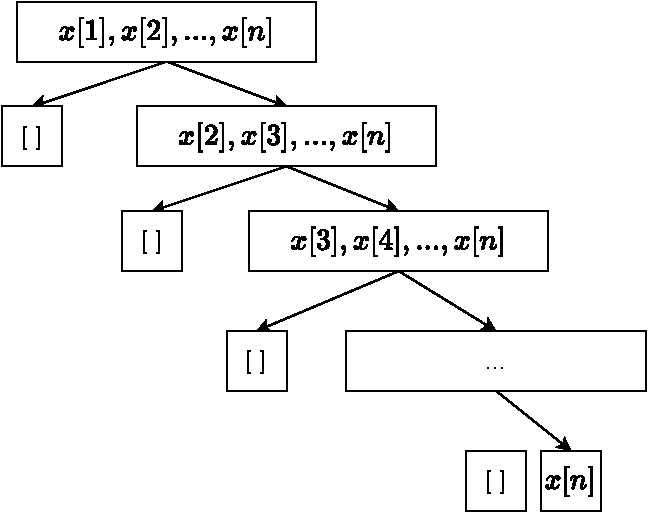
\includegraphics[scale=0.5]{img/unbalanced.ps}
    \caption{不平衡的树} \label{fig:unbalanced-tree}
\end{figure}


\begin{Exercise}
\Question{对于较大的通讯录,为了加快构建速度,有人使用两个并发的任务。一个任务从头部向后,另外一个任务从后向前读取。当两个任务在中间相遇时结束。这样构建出的二叉搜索树是什么样子的?如果把通讯录分成更多片断,使用更多的任务会得到什么结果?}
\Question{参考图\ref{fig:unbalanced-trees},找出更多的不平衡情况。}
\end{Exercise}

\begin{figure}[htbp]
  \centering
  \subcaptionbox{}{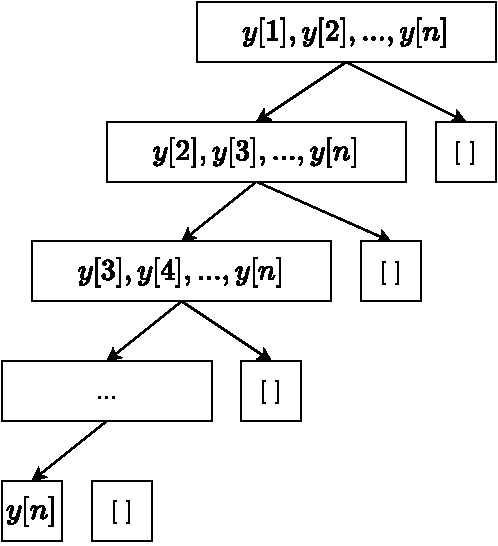
\includegraphics[scale=0.4]{img/unbalanced-2.ps}}
  \subcaptionbox{}{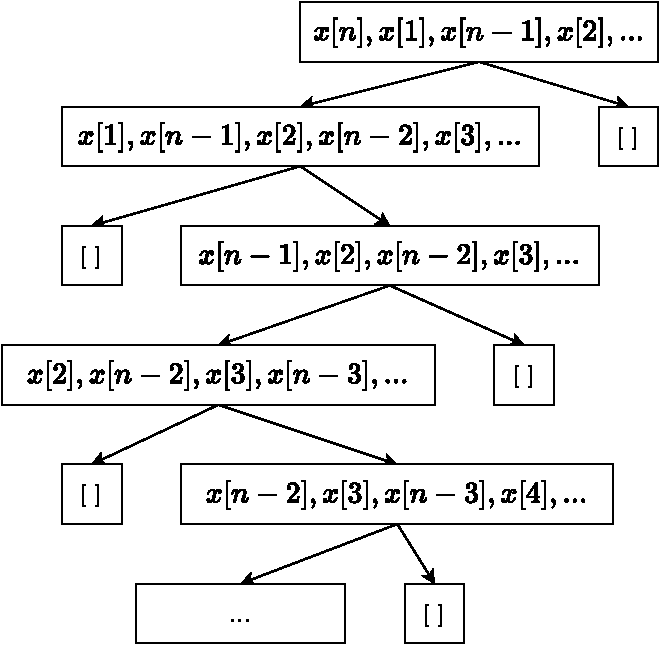
\includegraphics[scale=0.4]{img/unbalanced-zigzag.ps}} \\
  \subcaptionbox{}{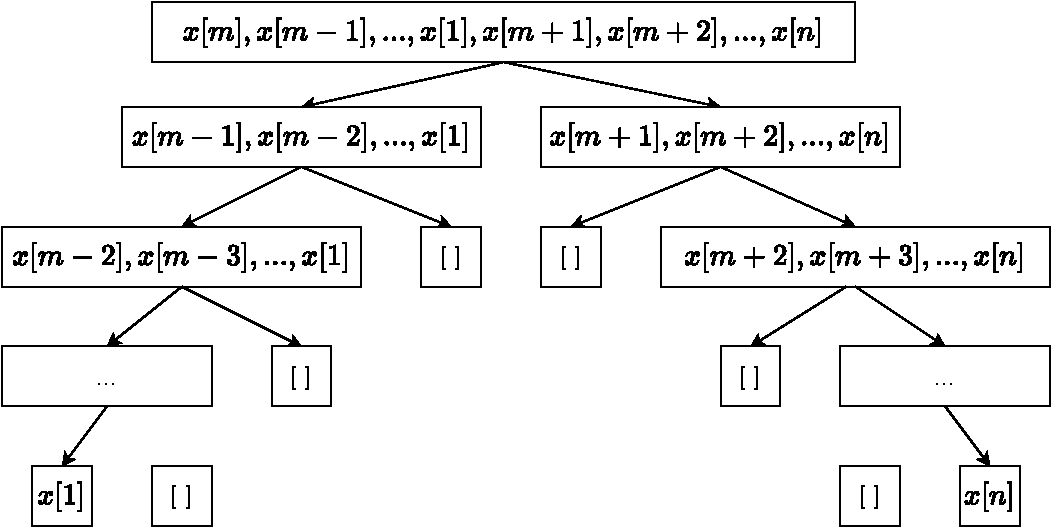
\includegraphics[scale=0.4]{img/unbalanced-3.ps}}
  \caption{一些不平衡的二叉树}
  \label{fig:unbalanced-trees}
\end{figure}

\subsection{平衡}

为了避免这种极不平衡的情况,我们可以将输入序列打乱(\cite{CLRS}第12.4节)。但这种方法有一定的局限性,如果序列是用户交互输入的,则无法应用这一方法。人们找到了一些解决平衡性的方法,它们大多依赖于二叉树的旋转操作。旋转操作可以在改变树结构的同时,保持元素间顺序不变。这一章介绍红黑树。它是一种被广泛使用的自平衡二叉搜索树。下一章我们介绍另外一种自平衡树――AVL树。第8章还会介绍伸展树,它能够随着操作,逐步把树变得平衡。

\subsection{树旋转}
\index{树旋转}

\begin{figure}[htbp]
  \centering
  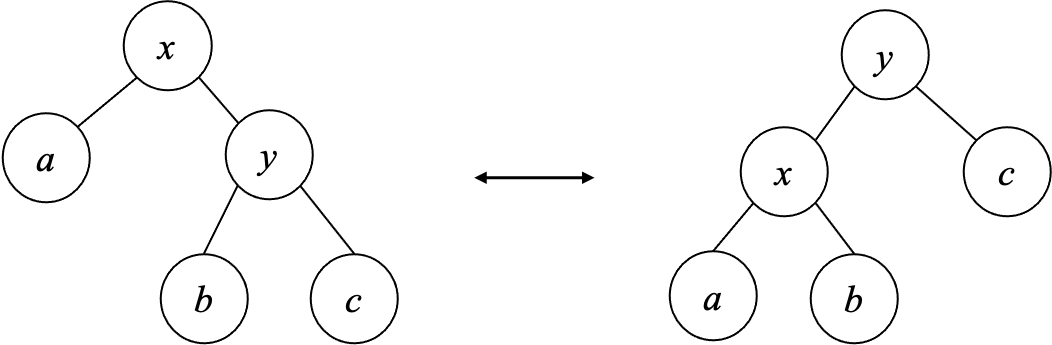
\includegraphics[scale=0.4]{img/tree-rotation.png}
  \caption{树的左右旋转}
  \label{fig:tree-rotation}
\end{figure}

树旋转在保持中序遍历结果不变的情况下,改变树的结构。存在多个不同的二叉树对应到一个特定的中序遍历顺序。图\ref{fig:tree-rotation}描述了旋转操作。

旋转操作可以通过模式匹配来定义:

\be
\begin{array}{rcl}
rotate_l\ ((a, x, b), y, c) & = & (a, x, (b, y, c)) \\
rotate_l\ T & = & T \\
\end{array}
\ee

和

\be
\begin{array}{rcl}
rotate_r\ (a, x, (b, y, c)) & = & ((a, x, b), y, c)) \\
rotate_r\ T & = & T \\
\end{array}
\ee

如果模式没有匹配(例如两棵子树都为空),每个式子的第二行保证树不变。旋转操作也可以通过一系列步骤实现。我们需要将子树和父引用设置正确。在旋转时,我们传入根节点$T$和要旋转的子树$x$:

\begin{algorithmic}[1]
\Function{Left-Rotate}{$T, x$}
  \State $p \gets$ \Call{Parent}{$x$}
  \State $y \gets$ \Call{Right}{$x$} \Comment{设$y \ne$ NIL}
  \State $a \gets$ \Call{Left}{$x$}
  \State $b \gets$ \Call{Left}{$y$}
  \State $c \gets$ \Call{Right}{$y$}
  \State \Call{Replace}{$x, y$}  \Comment{用$y$替换$x$}
  \State \Call{Set-Subtrees}{$x, a, b$} \Comment{令$a, b$为$x$的子树}
  \State \Call{Set-Subtrees}{$y, x, c$} \Comment{令$x, c$为$y$的子树}
  \If{$p = $ NIL}  \Comment{此前$x$是根节点}
    \State $T \gets y$
  \EndIf
  \State \Return $T$
\EndFunction
\end{algorithmic}

右旋\textproc{Right-Rotate}的实现是对称的,我们将其留作练习。\textproc{Replace}($x$, $y$)使用$y$替换$x$:

\begin{algorithmic}[1]
\Function{Replace}{$x, y$}
  \State $p \gets$ \Call{Parent}{$x$}
  \If{$p$ = NIL} \Comment{$x$是根节点}
    \If{$y \ne$ NIL}
           \Call{Parent}{$y$} $\gets$ NIL
    \EndIf
  \ElsIf{\Call{Left}{$p$} $= x$}
    \State \Call{Set-Left}{$p$, $y$}
  \Else
    \State \Call{Set-Right}{$p$, $y$}
  \EndIf
  \State \Call{Parent}{$x$} $\gets$ NIL
\EndFunction
\end{algorithmic}

\textproc{Set-Subtrees}($x, L, R$)将$L$设为$x$的左子树,$R$设为右子树:

\begin{algorithmic}[1]
\Function{Set-Subtrees}{$x, L, R$}
  \State \Call{Set-Left}{$x, L$}
  \State \Call{Set-Right}{$x, R$}
\EndFunction
\end{algorithmic}

它进一步调用\textproc{Set-Left}和\textproc{Set-Right}完成子树的设置:

\begin{algorithmic}[1]
\Function{Set-Left}{$x, y$}
  \State \Call{Left}{$x$} $\gets y$
  \If{$y \ne$ NIL}
    \Call{Parent}{$y$} $\gets x$
  \EndIf
  \EndFunction

\Statex

\Function{Set-Right}{$x, y$}
  \State \Call{Right}{$x$} $\gets y$
  \If{$y \ne$ NIL}
    \Call{Parent}{$y$} $\gets x$
  \EndIf
\EndFunction
\end{algorithmic}

通过对比,可以看到模式匹配如何简化树旋转的实现。从这一点出发Okasaki在1995年实现了红黑树的纯函数式算法\cite{okasaki}。

\begin{Exercise}
\Question{实现右旋\textproc{Right-Rotate}操作。}
\end{Exercise}

\section{定义}
\index{红黑树}

红黑树是一种自平衡二叉搜索树\cite{wiki-rbt}。它是2-3-4树的等价形式\footnote{第7章,B树。对于任一2-3-4树,都存在至少一棵红黑树,其元素顺序相同。}。通过对节点进行着色和旋转,红黑树可以高效地地保持平衡性。我们在二叉搜索树的定义上给节点赋予红、黑颜色。我们称一棵树为红黑树,如果它满足下面5条性质\cite{CLRS}:

\index{红黑树!红黑性质}
\begin{enumerate}
\item 节点的颜色为红色或黑色。
\item 根节点为黑色。
\item 所有的叶节点(NIL)为黑色。
\item 如果一个节点为红色,则它的两个子节点都是黑色。
\item 从任一节点出发到所有叶子节点的路径上包含相同数量的黑色节点。
\end{enumerate}

为什么这5条性质能保证红黑树的平衡性呢?关键在于:从根节点出发到达叶节点的所有路径中,最长路径不会超过最短路径两倍。性质4保证了不存在两个连续的红色节点。因此,最短的路径只含有黑色的节点。任何更长的路径一定含有红色节点。根据性质5,从任何节点出发的所有的路径都含有相同数量的黑色节点,自然这条对于根节点也成立。这就最终保证了没有任何路径超过最短路径长度的两倍\cite{wiki-rbt}。图\ref{fig:rbt-example-with-nil}的例子展示了一棵红黑树。

\begin{figure}[htbp]
  \centering
  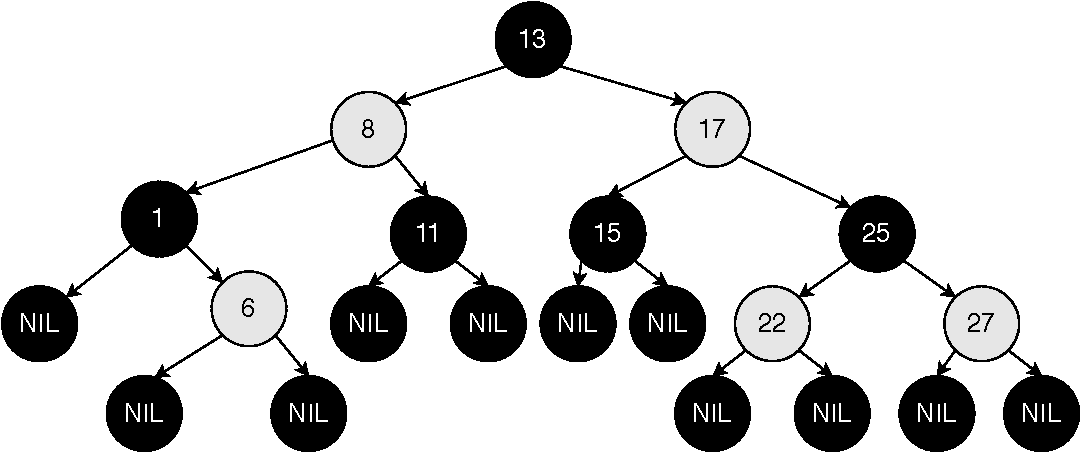
\includegraphics[scale=0.5]{img/rbt-example-with-nil.ps}
  \caption{红黑树}
  \label{fig:rbt-example-with-nil}
\end{figure}

由于所有的NIL节点都是黑色的,我们通常将NIL节点隐藏不画出,如图\ref{fig:rbt-example-with-nil}所示。所有不改变树结构的操作都和二叉搜索树相同,包括查找、最大、最小值等。只有插入和删除操作是特殊的。

\begin{figure}[htbp]
  \centering
  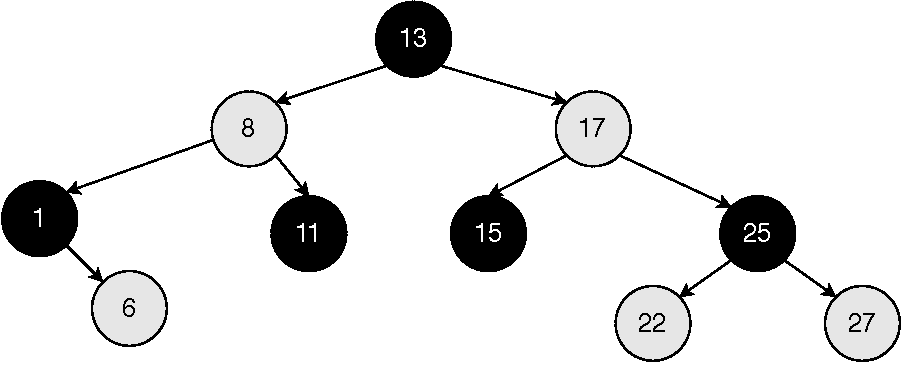
\includegraphics[scale=0.5]{img/rbt-example.ps}
  \caption{隐藏NIL节点}
  \label{fig:rbt-example}
\end{figure}

下面的例子程序在二叉搜索树的基础上增加了颜色定义:

\begin{Haskell}
data Color = R | B
data RBTree a = Empty
              | Node Color (RBTree a) a (RBTree a)
\end{Haskell}

\begin{Exercise}
\Question{证明含有$n$个节点的红黑树,其高度$h$不会超过$2 \lg (n+1)$。}
\end{Exercise}

\section{插入}
\index{红黑树!插入}

由于插入操作会改变树的结构,因此可能变得不平衡。为了保持红黑树的性质,我们需要在插入操作后进行变换来修复平衡问题。

当插入一个key时,我们可以把新节点一律染成红色。只要它不是根节点,除了第四条外的所有红黑树性质都可以满足。唯一的问题就是可能引入两个相邻的红色节点。

函数式和命令式实现使用不同的方法来修复平衡。前者直观简单,但是存在一点性能损失;后者有些复杂,但是具有更高的性能。大多数的算法书籍介绍后一种方法。本章中,我们关注函数式的方法,并展示这一方法极为简洁的特性。我们也会给出传统的命令式实现以作为对比。

Chris Okasaki指出,共有四种情况会违反红黑树的第四条性质。它们都带有两个相邻的红色节点。非常关键的一点是:它们可以被修复为一个统一形式\cite{okasaki},如图 \ref{fig:insert-fix}所示。

\begin{figure}[htbp]
  \centering
  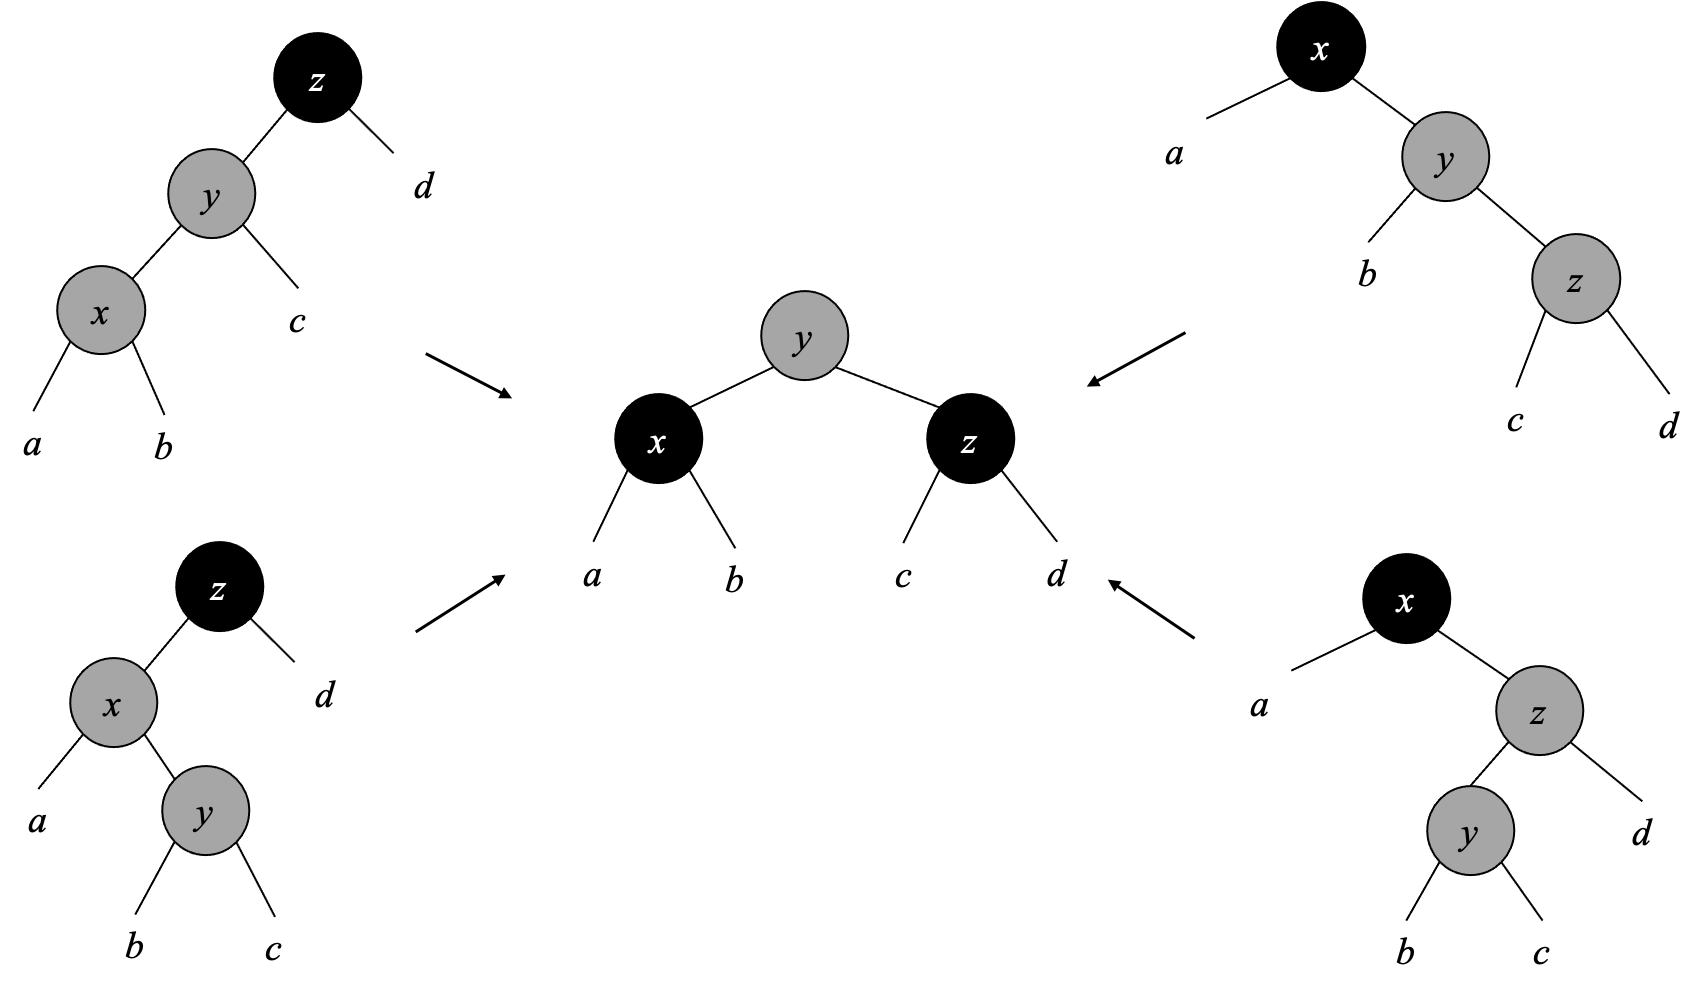
\includegraphics[scale=0.4]{img/insert-fix.png}
  \caption{插入后需要修复的四种情况}
  \label{fig:insert-fix}
\end{figure}

注意到这一变换会把红色向上“移动”一层。如果进行自底向上的递归修复,最后一步会把根节点染成红色。根据红黑树的第二条性质,根节点必须是黑色的。因此我们最后要把根节点再染回黑色。为了方便,我们把节点的颜色记为$\mathcal{C}$,它有两个值,黑色$\mathcal{B}$和红色$\mathcal{R}$。这样一棵非空的红黑树可以表达为一个四元组$T=(\mathcal{C}, T_l, k, T_r)$。

\be
balance(T) = \left \{
  \begin{array}
  {r@{\quad:\quad}l}
  (\mathcal{R}, (\mathcal{B}, A, x, B), y, (\mathcal{B}, C, z, D)) & match(T) \\
  T & otherwise
  \end{array}
\right .
\ee

其中,函数$match(T)$用以判断树是否符合图\ref{fig:insert-fix}中四种需要修复的情况。定义如下:

\[
match(T) : \left \{ T = \begin{array}{l}
         (\mathcal{B}, (\mathcal{R}, (\mathcal{R}, A, x, B), y, C), z, D) \lor \\
         (\mathcal{B}, (\mathcal{R}, A, x, (\mathcal{R}, B, y, C), z, D)) \lor \\
         (\mathcal{B}, A, x, (\mathcal{R}, B, y, (\mathcal{R}, C, z, D))) \lor \\
         (\mathcal{B}, A, x, (\mathcal{R}, (\mathcal{R}, B, y, C), z, D)) \\
         \end{array} \right \}
\]

定义好函数$balance(T)$后,我们就可以修改二叉搜索树的插入函数,使其支持红黑树。

\be
insert(T, k) = makeBlack(ins(T, k))
\ee

其中$ins(T, k)$函数定义如下:

\be
ins(T, k) = \left \{
  \begin{array}
  {r@{\quad:\quad}l}
  (\mathcal{R}, \phi, k, \phi) & T = \phi \\
  balance((ins(T_l, k), k', T_r)) & k < k' \\
  balance((T_l, k', ins(T_r, k))) & otherwise
  \end{array}
\right.
\ee

如果待插入的树为空,则创建一个新的红色节点,节点的key就是待插入的$k$;否则,记树的左右分支和key分别为$T_l$、$T_r$和$k'$,我们比较$k$和$k'$的大小,递归地将它插入子分支中,然后再用$balance$函数恢复平衡。最后,我们使用$makeBlack(T)$函数把根节点染成黑色。

\be
makeBlack(T) = (\mathcal{B}, T_l, k, T_r)
\ee

在支持模式匹配的语言中,例如Haskell,插入算法可以实现为下面的程序:

\lstset{language=Haskell}
\begin{lstlisting}[style=Haskell]
insert t x = makeBlack $ ins t where
    ins Empty = Node R Empty x Empty
    ins (Node color l k r)
        | x < k     = balance color (ins l) k r
        | otherwise = balance color l k (ins r) --[3]
    makeBlack(Node _ l k r) = Node B l k r

balance B (Node R (Node R a x b) y c) z d =
                Node R (Node B a x b) y (Node B c z d)
balance B (Node R a x (Node R b y c)) z d =
                Node R (Node B a x b) y (Node B c z d)
balance B a x (Node R b y (Node R c z d)) =
                Node R (Node B a x b) y (Node B c z d)
balance B a x (Node R (Node R b y c) z d) =
                Node R (Node B a x b) y (Node B c z d)
balance color l k r = Node color l k r
\end{lstlisting} %$

程序中的\texttt{balance}函数略微有些不同,它的参数不是一棵树,而是节点的颜色、左侧分支、key和右侧分支。这样可以节省一对boxing和unboxing的操作。

我们没有处理存在重复key的情况。如果发生重复,我们可以选择覆盖,或者跳过不处理,还可以在节点中用一个链表存储重复的数据(\cite{CLRS}, 第269页)。

图\ref{fig:insert-example}中给出了两个插入的例子。左侧是依次将11, 2, 14, 1, 7, 5, 8, 4插入的结果。右侧的是将序列1, 2, ..., 8插入的结果。可以看到,即使输入已序序列,红黑树仍然保持平衡。

\begin{figure}[htbp]
  \centering
  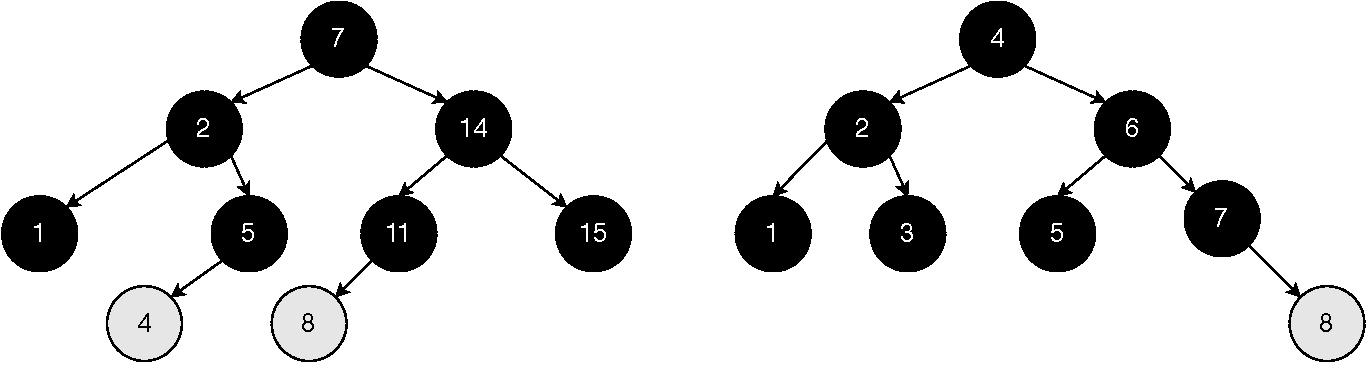
\includegraphics[scale=0.5]{img/insert-haskell.ps}
  \caption{根据不同的序列,使用插入算法产生的两棵红黑树} \label{fig:insert-example}
\end{figure}

通过将四种不同的情况统一变换成同一种形式,我们得到了一个极为简洁的算法。即使在不支持模式匹配的语言中,我们仍然可以编程检验树是否满足一定的模式。这样得到的结果和传统方法相比,仍然会简洁很多。读者可以参考本章附带的Lisp方言Scheme的例子代码。

对于含有$n$个节点的红黑树,这一插入算法的复杂度为$O(\lg n)$。

\begin{Exercise}

\begin{itemize}
\item 使用一种命令式语言,例如C、C++或Python来实现本节介绍的插入算法。注意:如果语言本身不支持模式匹配,需要编程检查四种不同的情况。
\end{itemize}

\end{Exercise}

% ================================================================
%                 Deletion
% ================================================================

\section{删除}
\index{红黑树!删除}

上一章曾指出,二叉搜索树的删除操作只在命令式环境下才有意义。这一结论同样适用于红黑树。大多数情况下,通常一次性将树构建好,然后频繁地进行查找。Okasaki曾经解释过为什么他没有给出红黑树的删除算法\cite{okasaki-blog}。其中一个原因就是删除比插入要麻烦得多。

我们希望通过本节的介绍,使读者了解到,在纯函数式的环境中,删除算法是可以实现的。纯函数式数据结构决定了树不会真的被改变,我们实际上是重建了一棵树\footnote{大多数函数式编程环境通过使用一种名为persistent的技术,可以复用树中没有改变的部分,从而减小重建的开销。}。实际应用中,往往是由用户(也就是编程者)来决定使用那种具体的方案。例如,我们可以不做任何操作,而仅仅标记一下要删除的节点。当带有删除标记的节点超过50\%的时候,用所有未标记的节点重建一棵树。

不仅是函数式环境,命令式的删除算法也比插入算法要复杂。这主要是因为在删除时,我们面临更多的情况需要修复平衡。删除也会破坏红黑树的性质,因此需要后继的处理以恢复平衡。

本节介绍的删除算法主要来自\cite{lyn}。只有在删除一个黑色的节点时才会引发问题。因为这样会破坏红黑树的第五条性质,使得某一路径上的黑色节点数目少于其他的路径。

在删除一个黑色节点时,我们可以通过引入“双重黑色”\cite{CLRS}的概念来恢复第五条性质。也就是说,虽然节点被删除了,我们把它的黑色保存在它的父节点中。如果父节点是红色的,我们将其变为黑色;但如果父节点已经是黑色的,它就会变成一个“双重黑色”的节点。

为了使用双重黑色概念,我们需要修改一下红黑树的定义,如下面的Haskell示例代码:

\lstset{language=Haskell}
\begin{lstlisting}[style=Haskell]
data Color = R | B | BB -- BB: 用于删除操作的双重黑色
data RBTree a = Empty | BBEmpty -- 双重黑色的空节点
              | Node Color (RBTree a) a (RBTree a)
\end{lstlisting}

删除一个节点时,我们先调用普通二叉搜索树的删除算法。如果被删除节点是黑色的,我们接下来进行修复。删除函数定义如下:

\be
delete(T, k) = blackenRoot(del(T, k))
\ee

其中

\be
del(T, k) = \left \{
  \begin{array}
  {r@{\quad:\quad}l}
  \phi & T = \phi \\
  fixBlack^2((\mathcal{C}, del(T_l, k), k', T_r)) & k < k' \\
  fixBlack^2((\mathcal{C}, T_l, k', del(T_r, k))) & k > k' \\
  \left \{
    \begin{array}{r@{\quad:\quad}l}
    mkBlk(T_r) & \mathcal{C} = \mathcal{B} \\
    T_r & otherwise
    \end{array}
  \right. & T_l = \phi \\
  \left \{
    \begin{array}{r@{\quad:\quad}l}
    mkBlk(T_l) & \mathcal{C} = \mathcal{B} \\
    T_l & otherwise
    \end{array}
  \right.  & T_r = \phi \\
  fixBlack^2((\mathcal{C}, T_l, k'', del(T_r, k''))) & otherwise
  \end{array}
\right.
\ee

函数$del$定义了各种不同的情况。如果树为空,这种边界情况下的删除结果也为空$\phi$;否则,如果待删除的key比当前节点的key小,我们递归地在左侧分支进行删除;如果比当前节点的key大,则递归地在右侧分支删除。由于可能引入双重黑色,所以需要后继的修复处理。

如果待删除的key恰好等于当前节点的key,我们需要将其“切下”。若当前节点有一个子分支为空,我们只要用另外一个分支替换当前节点,并且保持当前节点的颜色属性就可以了。否则,如果两个分支都不为空,我们从右侧子分支中找到最小值$k''=min(T_r)$,将其“切下”并替换掉当前的节点的key。

最后,函数$delete$通过调用$blackenRoot$强制将根节点染成黑色。

\be
blackenRoot(T) = \left \{
  \begin{array}
  {r@{\quad:\quad}l}
  \phi & T = \phi \\
  (\mathcal{B}, T_l, k, T_r) & otherwise \\
  \end{array}
\right .
\ee

和红黑树插入算法中的$makeBlack$函数相比,$blackenRoot$仅仅多了对为空树的处理。这一处理仅在删除时才需要考虑,因为插入操作不可能产生一棵空树,而删除操作是有可能的。

函数$mkBlk$用于保持被“切下”节点的黑色属性。如果被“切下”的节点为黑色,它将红色的结果改为黑色,把黑色的结果改为双重黑色。如果结果为空,则将其标记为双重黑色的空,记为$\Phi$。

\be
mkBlk(T) = \left \{
  \begin{array}
  {r@{\quad:\quad}l}
  \Phi & T = \phi \\
  (\mathcal{B}, T_l, k, T_r) & \mathcal{C} = \mathcal{R} \\
  (\mathcal{B}^2, T_l, k, T_r) & \mathcal{C} = \mathcal{B} \\
  T & otherwise
  \end{array}
\right .
\ee

其中,符号$\mathcal{B}^2$表示双重黑色。

将目前的函数定义翻译为Haskell可以得到下面的例子程序。

\begin{lstlisting}[style=Haskell]
delete t x = blackenRoot(del t x) where
    del Empty _ = Empty
    del (Node color l k r) x
        | x < k = fixDB color (del l x) k r
        | x > k = fixDB color l k (del r x)
        -- x == k, 删除此节点
        | isEmpty l = if color==B then makeBlack r else r
        | isEmpty r = if color==B then makeBlack l else l
        | otherwise = fixDB color l k' (del r k') where k'= min r
    blackenRoot (Node _ l k r) = Node B l k r
    blackenRoot _ = Empty

makeBlack (Node B l k r) = Node BB l k r -- 双重黑色
makeBlack (Node _ l k r) = Node B l k r
makeBlack Empty = BBEmpty
makeBlack t = t
\end{lstlisting}

删除算法中,唯一还没有定义的函数是$fixBlack^2$。我们需要在这个函数中,通过树的旋转操作和重新染色,最终去掉“双重黑色”。这里有三种情况需要处理。每一种情况中,双重黑色的节点即可以是普通节点,也可以是双重黑色的空节点$\Phi$。我们首先看第一种情况。

\subsection{双重黑色节点的兄弟为黑色,并且该兄弟节点有一个红色子节点}
对于这种情况,我们可以通过旋转操作来修复。总共有四种不同的细分情况,它们全部可以变换到一种统一的形式。如图\ref{fig:del-case1}所示。

\begin{figure}[htbp]
   \centering
   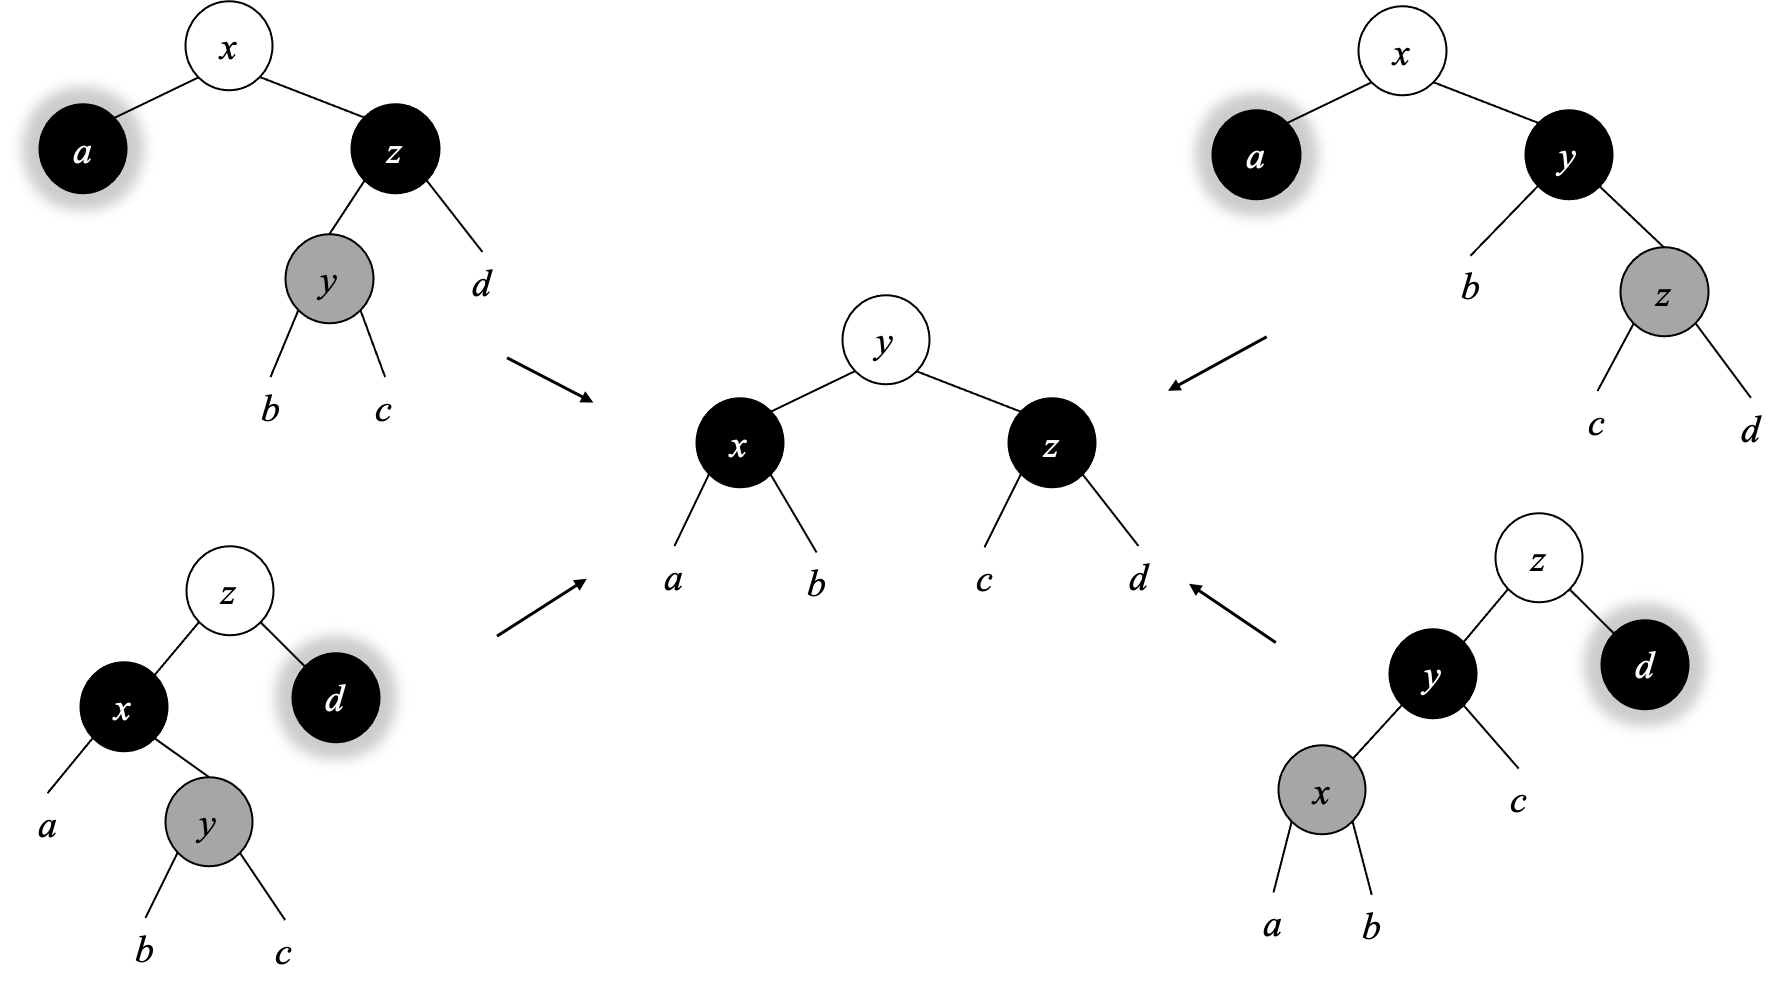
\includegraphics[scale=0.4]{img/del-case1.png}
   \caption{4种细分情况可以用共同的方法修复}
   \label{fig:del-case1}
\end{figure}

我们通过模式匹配来处理这四种细分情况:

\be
fixBlack^2(T) = \left \{
  \begin{array}
  {r@{\quad:\quad}l}
  (\mathcal{C}, (\mathcal{B}, mkBlk(A), x, B), y, (\mathcal{B}, C, z, D)) & p 1.1 \\
  (\mathcal{C}, (\mathcal{B}, A, x, B), y, (\mathcal{B}, C, z, mkBlk(D))) & p 1.2 \\
  \end{array}
\right .
\label{eq:db-case-1}
\ee

其中$p 1.1$和$p 1.2$各代表两种细分情况:

\[
p 1.1 : \left \{ \begin{array}{l}
  T = (\mathcal{C}, A, x, (\mathcal{B}, (\mathcal{R}, B, y, C), z, D)) \land color(A) = \mathcal{B}^2 \\
  \lor \\
  T = (\mathcal{C}, A, x, (\mathcal{B}, B, y, (\mathcal{R}, C, z, D))) \land color(A) = \mathcal{B}^2
  \end{array} \right \}
\]

\[
p 1.2 : \left \{ \begin{array}{l}
  T = (\mathcal{C}, (\mathcal{B}, A, x, (\mathcal{R}, B, y, C)), z, D) \land color(D) = \mathcal{B}^2 \\
  \lor \\
  T = (\mathcal{C}, (\mathcal{B}, (\mathcal{R}, A, x, B), y, C), z, D) \land color(D) = \mathcal{B}^2
  \end{array} \right \}
\]

如果双重黑色的节点是双重黑色空节点$\Phi$,经过这样的旋转操作后,可以将其恢复为普通空节点。为此我们为式\ref{eq:db-case-1}增加双重黑色空节点的处理:

\be
fixBlack^2(T) = \left \{
  \begin{array}
  {r@{\quad:\quad}l}
  (\mathcal{C}, (\mathcal{B}, mkBlk(A), x, B), y, (\mathcal{B}, C, z, D)) & p 1.1 \\
  (\mathcal{C}, (\mathcal{B}, \phi, x, B), y, (\mathcal{B}, C, z, D)) & p 1.1' \\
  (\mathcal{C}, (\mathcal{B}, A, x, B), y, (\mathcal{B}, C, z, mkBlk(D))) & p 1.2 \\
  (\mathcal{C}, (\mathcal{B}, A, x, B), y, (\mathcal{B}, C, z, \phi)) & p 1.2' \\
  \end{array}
\right .
\label{eq:db-case-1a}
\ee

其中$p 1.1'$和$p 1.2'$的模式定义如下:

\[
p 1.1' : \left \{ \begin{array}{l}
  T = (\mathcal{C}, \Phi, x, (\mathcal{B}, (\mathcal{R}, B, y, C), z, D)) \\
  \lor \\
  T = (\mathcal{C}, \Phi, x, (\mathcal{B}, B, y, (\mathcal{R}, C, z, D)))
  \end{array} \right \}
\]

\[
p 1.2' : \left \{ \begin{array}{l}
  T = (\mathcal{C}, (\mathcal{B}, A, x, (\mathcal{R}, B, y, C)), z, \Phi) \\
  \lor \\
  T = (\mathcal{C}, (\mathcal{B}, (\mathcal{R}, A, x, B), y, C), z, \Phi)
  \end{array} \right \}
\]

\subsection{双重黑色节点的兄弟节点为红色}
这种情况下,我们可以通过旋转,将其变换为$p 1.1$和$p 1.2$。如图\ref{fig:del-case2}所示。

\begin{figure}[htbp]
  \centering
  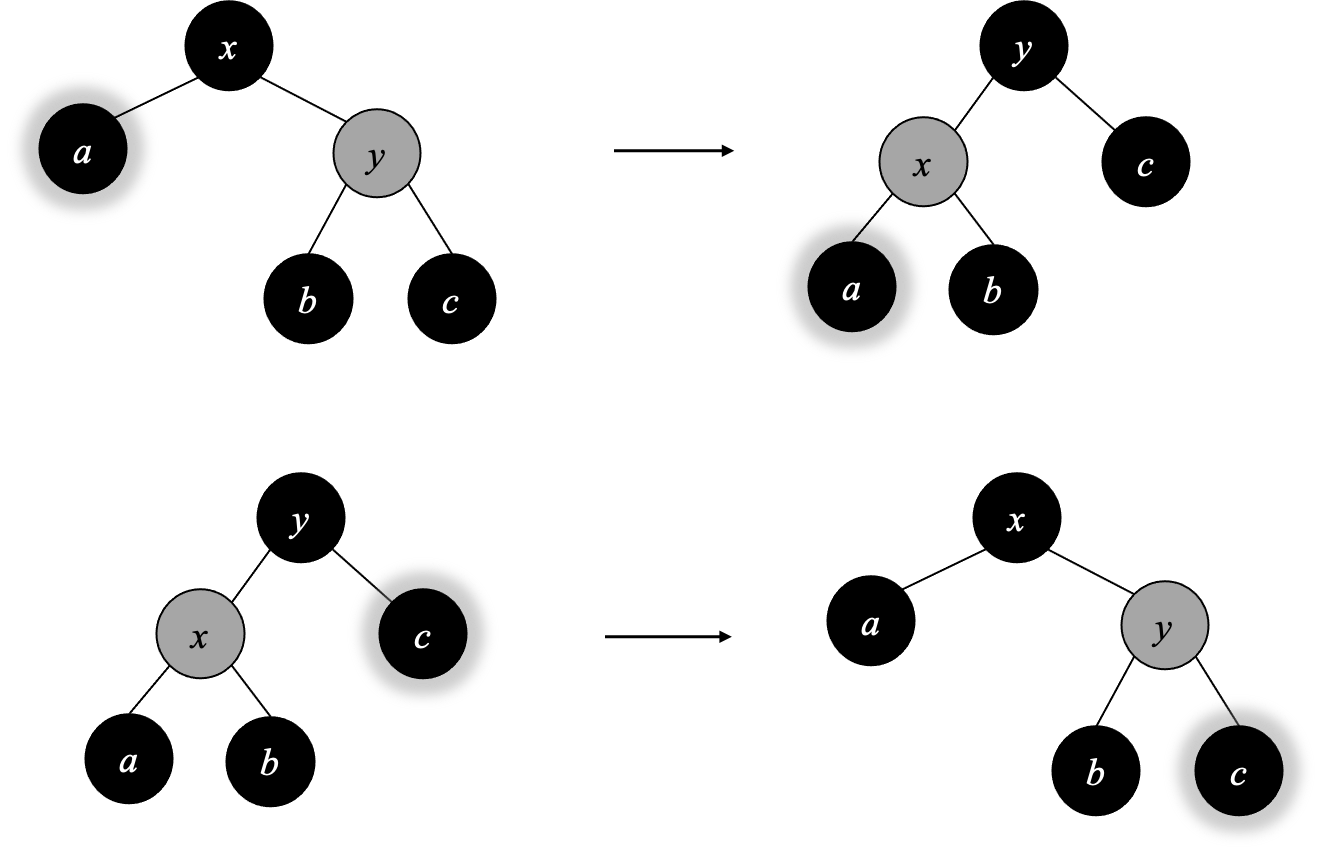
\includegraphics[scale=0.4]{img/del-case2.png}
  \caption{双重黑色节点的兄弟节点为红色} \label{fig:del-case2}
\end{figure}

在公式(\ref{eq:db-case-1a})的基础上增加这一处理可以得到公式(\ref{eq:db-case-2})。

\be
fixBlack^2(T) = \left \{
  \begin{array}
  {r@{\quad:\quad}l}
  ... & ... \\
  fixBlack^2(\mathcal{B}, fixBlack^2((\mathcal{R}, A, x, B), y, C) & p 2.1 \\
  fixBlack^2(\mathcal{B}, A, x, fixBlack^2((\mathcal{R}, B, y, C)) & p 2.2 \\
  T & otherwise
  \end{array}
\right .
\label{eq:db-case-2}
\ee

其中$p 2.1$和$p 2.2$表示如下:

\[
p 2.1 : \{ color(T) = \mathcal{B} \land color(T_l) = \mathcal{B}^2 \land color(T_r) = \mathcal{R} \}
\]

\[
p 2.2 : \{ color(T) = \mathcal{B} \land color(T_l) = \mathcal{R} \land color(T_r) = \mathcal{B}^2 \}
\]

\subsection{双重黑色节点的兄弟节点为黑色,该兄弟节点的两个子节点也全是黑色。}
这种情况下,我们可以将这个兄弟节点染成红色,将双重黑色变回黑色,然后将双重黑色属性向上传递一层到父节点。如图\ref{fig:del-case3}所示,有两种对称的情况。

\begin{figure}[htbp]
  \centering
  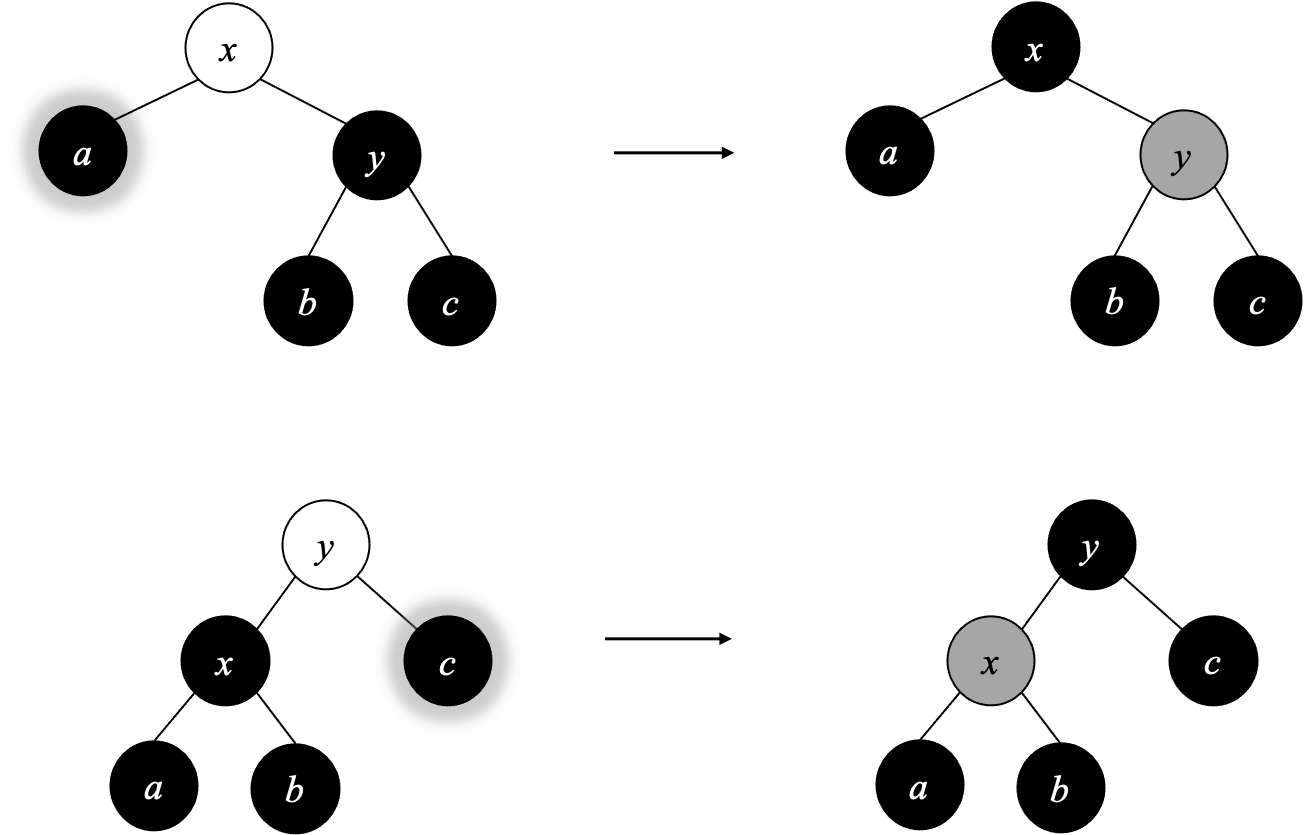
\includegraphics[scale=0.4]{img/del-case3.png}
  \caption{将双重黑色向上传递} \label{fig:del-case3}
\end{figure}

我们继续在式(\ref{eq:db-case-2})的基础上增加修复的定义。

\be
fixBlack^2(T) = \left \{
  \begin{array}
  {r@{\quad:\quad}l}
  ... & ... \\
  mkBlk((\mathcal{C}, mkBlk(A), x, (\mathcal{R}, B, y, C))) & p 3.1 \\
  mkBlk((\mathcal{C}, (\mathcal{R}, A, x, B), y, mkBlk(C))) & p 3.2 \\
  ... & ...
  \end{array}
\right .
\label{eq:db-case-3}
\ee

其中$p 3.1$和$p 3.2$定义如下:

\[
p 3.1 : \left \{ \begin{array}{l}
  T = (\mathcal{C}, A, x, (\mathcal{B}, B, y, C)) \land \\
  color(A) = \mathcal{B}^2 \land color(B) = color(C) = \mathcal{B}
  \end{array} \right \}
\]

\[
p 3.2 : \left \{ \begin{array}{l}
  T = (\mathcal{C}, (\mathcal{B}, A, x, B), y, C) \land \\
  color(C) = \mathcal{B}^2 \land color(A) = color(B) = \mathcal{B}
  \end{array} \right \}
\]

如果双重黑色的节点是双重黑色空节点$\Phi$,经过重新染色后,可以将其恢复为普通空节点。我们在式\ref{eq:db-case-3}的基础上增加双重黑色空节点的处理:

\be
fixBlack^2(T) = \left \{
  \begin{array}
  {r@{\quad:\quad}l}
  ... & ... \\
  mkBlk((\mathcal{C}, mkBlk(A), x, (\mathcal{R}, B, y, C))) & p 2.1 \\
  mkBlk((\mathcal{C}, \phi, x, (\mathcal{R}, B, y, C))) & p 2.1' \\
  mkBlk((\mathcal{C}, (\mathcal{R}, A, x, B), y, mkBlk(C))) & p 2.2 \\
  mkBlk((\mathcal{C}, (\mathcal{R}, A, x, B), y, \phi)) & p 2.2' \\
  ... & ...
  \end{array}
\right .
\label{eq:db-case-3a}
\ee

其中$p 3.1'$和$p 3.2'$定义如下:

\[
p 3.1' : \left \{ \begin{array}{l}
  T = (\mathcal{C}, \Phi, x, (\mathcal{B}, B, y, C)) \land \\
  color(B) = color(C) = \mathcal{B}
  \end{array} \right \}
\]

\[
p 3.2' : \left \{ \begin{array}{l}
  T = (\mathcal{C}, (\mathcal{B}, A, x, B), y, \Phi) \land \\
  color(A) = color(B) = \mathcal{B}
  \end{array} \right \}
\]

至此,我们对于双重黑色的全部情况都完成了修复。算法被定义为一个递归函数。它有两个终止条件:一个是$p1.1$和$p1.2$,双重黑色节点被直接消除了;另外一个是将双重黑色继续向上传递,直到根节点。由于算法最终会将根节点染成黑色,所以双重黑色也会被消除。

综合公式(\ref{eq:db-case-1a})、(\ref{eq:db-case-2})和(\ref{eq:db-case-3a}),我们可以得到最终的Haskell删除程序。

\begin{lstlisting}[style=Haskell]
-- 兄弟节点为黑色,并且有一个红色子节点
fixDB color a@(Node BB _ _ _) x (Node B (Node R b y c) z d)
      = Node color (Node B (makeBlack a) x b) y (Node B c z d)
fixDB color BBEmpty x (Node B (Node R b y c) z d)
      = Node color (Node B Empty x b) y (Node B c z d)
fixDB color a@(Node BB _ _ _) x (Node B b y (Node R c z d))
      = Node color (Node B (makeBlack a) x b) y (Node B c z d)
fixDB color BBEmpty x (Node B b y (Node R c z d))
      = Node color (Node B Empty x b) y (Node B c z d)
fixDB color (Node B a x (Node R b y c)) z d@(Node BB _ _ _)
      = Node color (Node B a x b) y (Node B c z (makeBlack d))
fixDB color (Node B a x (Node R b y c)) z BBEmpty
      = Node color (Node B a x b) y (Node B c z Empty)
fixDB color (Node B (Node R a x b) y c) z d@(Node BB _ _ _)
      = Node color (Node B a x b) y (Node B c z (makeBlack d))
fixDB color (Node B (Node R a x b) y c) z BBEmpty
      = Node color (Node B a x b) y (Node B c z Empty)
-- 兄弟节点是红色
fixDB B a@(Node BB _ _ _) x (Node R b y c) = fixDB B (fixDB R a x b) y c
fixDB B a@BBEmpty x (Node R b y c) = fixDB B (fixDB R a x b) y c
fixDB B (Node R a x b) y c@(Node BB _ _ _) = fixDB B a x (fixDB R b y c)
fixDB B (Node R a x b) y c@BBEmpty = fixDB B a x (fixDB R b y c)
-- 兄弟节点和它的两个子节点都是黑色,向上传递黑色
fixDB color a@(Node BB _ _ _) x (Node B b y c) = makeBlack (Node color (makeBlack a) x (Node R b y c))
fixDB color BBEmpty x (Node B b y c) = makeBlack (Node color Empty x (Node R b y c))
fixDB color (Node B a x b) y c@(Node BB _ _ _) = makeBlack (Node color (Node R a x b) y (makeBlack c))
fixDB color (Node B a x b) y BBEmpty = makeBlack (Node color (Node R a x b) y Empty)
-- 其他情况
fixDB color l k r = Node color l k r
\end{lstlisting}

对于含有$n$个节点的红黑树,删除算法的复杂度为$O(\lg n)$。

\begin{Exercise}

\begin{itemize}
\item 选用一种编程语言,实现本节提到的“标记――重建”删除算法:也就是先将要删除的节点标记,但不进行真正的删除。当被标记的节点数目超过50\%的时候,用全部未标记的节点重建树。
\item 为什么不需要在$mkBlk$的调用处,显示地再调用$fixBlack^2$?
\end{itemize}

\end{Exercise}

\section{命令式的红黑树算法$\star$}
\index{红黑树!命令式插入}

通过归纳,我们能够简洁地实现红黑树算法。作为对比,我们来看一下传统的命令式方法。

插入算法的基本思想仍然和二叉搜索树相同。此外,算法需要通过树的旋转操作修复平衡。

\begin{algorithmic}[1]
\Function{Insert}{$T, k$}
  \State $root \gets T$
  \State $x \gets$ \Call{Create-Leaf}{$k$}
  \State \Call{Color}{$x$} $\gets$ RED
  \State $p \gets$ NIL
  \While{$T \neq$ NIL}
    \State $p \gets T$
    \If{$k <$ \Call{Key}{$T$}}
      \State $T \gets $ \Call{Left}{$T$}
    \Else
      \State $T \gets $ \Call{Right}{$T$}
    \EndIf
  \EndWhile
  \State \Call{Parent}{$x$} $\gets p$
  \If{$p =$ NIL} \Comment{树$T$为空}
    \State \Return $x$
  \ElsIf{$k <$ \Call{Key}{$p$}}
    \State \Call{Left}{$p$} $\gets x$
  \Else
    \State \Call{Right}{$p$} $\gets x$
  \EndIf
  \State \Return \Call{Insert-Fix}{$root, x$}
\EndFunction
\end{algorithmic}

当插入一个新节点时,我们将其染成红色,然后修复平衡并返回。上述算法可以转换为下面的Python例子程序。

\lstset{language=Python}
\begin{lstlisting}
def rb_insert(t, key):
    root = t
    x = Node(key)
    parent = None
    while(t):
        parent = t
        if(key < t.key):
            t = t.left
        else:
            t = t.right
    if parent is None: #树为空
        root = x
    elif key < parent.key:
        parent.set_left(x)
    else:
        parent.set_right(x)
    return rb_insert_fix(root, x)
\end{lstlisting}

总共有3种基本情况需要修复。如果考虑左右对称,则需要修复6种情况。3种基本情况中的两种可以合并。新插入节点的父节点,以及父节点的兄弟节点均为红色。我们可以把它们变为黑色,然后把新插入节点的祖父节点染为红色。修复算法的实现如下:

\begin{algorithmic}[1]
\Function{Insert-Fix}{$T, x$}
  \While{\Call{Parent}{$x$} $\neq$ NIL $\land$ \textproc{Color}(\Call{Parent}{$x$}) = RED}
    \If{\textproc{Color}(\Call{Uncle}{$x$}) $=$ RED}
      \Comment{情况1:$x$的叔父节点是红色}
      \State \textproc{Color}(\Call{Parent}{$x$}) $\gets$ BLACK
      \State \textproc{Color}(\Call{Grand-Parent}{$x$}) $\gets$ RED
      \State \textproc{Color}(\Call{Uncle}{$x$}) $\gets$ BLACK
      \State $x \gets$ \Call{Grand-Parent}{$x$}
    \Else
      \Comment{$x$的叔父节点是黑色}
      \If{\Call{Parent}{$x$} = \textproc{Left}(\Call{Grand-Parent}{$x$})}
        \If{ $x =$ \textproc{Right}(\Call{Parent}{$x$})}
          \Comment{情况2:$x$是右侧子节点}
          \State $x \gets$ \Call{Parent}{$x$}
          \State $T \gets$ \Call{Left-Rotate}{$T, x$}
        \EndIf
        \Comment{情况3:$x$是左侧子节点}
        \State \textproc{Color}(\Call{Parent}{$x$}) $\gets$ BLACK
        \State \textproc{Color}(\Call{Grand-Parent}{$x$}) $\gets$ RED
        \State $T \gets$ \textproc{Right-Rotate}($T$, \Call{Grand-Parent}{$x$})
      \Else
         \If{ $x =$ \textproc{Left}(\Call{Parent}{$x$})}
          \Comment{情况2的对称情况}
          \State $x \gets$ \Call{Parent}{$x$}
          \State $T \gets$ \Call{Right-Rotate}{$T, x$}
        \EndIf
        \Comment{情况3的对称情况}
        \State \textproc{Color}(\Call{Parent}{$x$}) $\gets$ BLACK
        \State \textproc{Color}(\Call{Grand-Parent}{$x$}) $\gets$ RED
        \State $T \gets$ \textproc{Left-Rotate}($T$, \Call{Grand-Parent}{$x$})
      \EndIf
    \EndIf
  \EndWhile
  \State \Call{Color}{$T$} $\gets$ BLACK
  \State \Return $T$
\EndFunction
\end{algorithmic}

这一算法向红黑树中插入key的复杂度为$O(\lg n)$。和前面定义的$balance$函数相比,我们可以发现它们的差异。两种方法不仅仅在篇幅长短上不同,具体的逻辑也不一样。即使输入同一序列的key,两种方法也会构造出不同的红黑树。并且,和这一命令式算法相比,前面使用模式匹配的函数式算法存在一些性能上的损失。Okasaki在\cite{okasaki}中给出了关于函数式红黑树插入算法性能的详细分析。

上述修复算法可以实现为如下的Python例子程序。

\lstset{language=Python}
\begin{lstlisting}
# 修复连续的红色节点
def rb_insert_fix(t, x):
    while(x.parent and x.parent.color==RED):
        if x.uncle().color == RED:
            # 情况1: ((a:R x:R b) y:B c:R) ==> ((a:R x:B b) y:R c:B)
            set_color([x.parent, x.grandparent(), x.uncle()],
                      [BLACK, RED, BLACK])
            x = x.grandparent()
        else:
            if x.parent == x.grandparent().left:
                if x == x.parent.right:
                    # 情况2: ((a x:R b:R) y:B c) ==> 情况3
                    x = x.parent
                    t=left_rotate(t, x)
                # 情况3: ((a:R x:R b) y:B c) ==> (a:R x:B (b y:R c))
                set_color([x.parent, x.grandparent()], [BLACK, RED])
                t=right_rotate(t, x.grandparent())
            else:
                if x == x.parent.left:
                    # 情况2': (a x:B (b:R y:R c)) ==> 情况3'
                    x = x.parent
                    t = right_rotate(t, x)
                # 情况3': (a x:B (b y:R c:R)) ==> ((a x:R b) y:B c:R)
                set_color([x.parent, x.grandparent()], [BLACK, RED])
                t=left_rotate(t, x.grandparent())
    t.color = BLACK
    return t
\end{lstlisting}

图\ref{fig:imperative-insert}给出了两棵红黑树,它们是使用和图\ref{fig:insert-example}中完全相同的序列构造出的。我们可以发现它们明显不同。

\begin{figure}[htbp]
   \centering
   \subcaptionbox{}{\includegraphics[scale=0.4]{img/clrs-fig-13-4.ps}}
   \subcaptionbox{}{\includegraphics[scale=0.4]{img/python-insert.ps}}
   \caption{命令式算法构建出的红黑树}
   \label{fig:imperative-insert}
\end{figure}

红黑树的命令式删除算法和插入算法相比更为复杂。我们不在正文给出,读者可以参考本书附录B了解其详细实现。

\section{其它}
红黑树是最广泛使用的一种平衡二叉搜索树。另外一种自平衡二叉树是AVL树,我们将在下一章介绍。红黑树可以帮助我们了解其它更复杂的数据结构。如果我们将子节点的数目从两个扩展到$k$个,并且保持树的平衡,就可以演化到B树。如果我们在边上,而非在节点中存储数据,我们就得到了Trie。由于常见红黑树算法需要处理很多情况,代码篇幅较长,初学者往往会感觉红黑树很复杂。

Okasaki的工作使得红黑树算法变得容易理解。这激发了很多其它程序设计语言进行类似的实现\cite{rosetta}。本书中给出的Splay树、AVL树等模式匹配算法也是受到这一启发而完成的。

\ifx\wholebook\relax \else
\begin{thebibliography}{99}

\bibitem{CLRS}
Thomas H. Cormen, Charles E. Leiserson, Ronald L. Rivest and Clifford Stein.
``Introduction to Algorithms, Second Edition''. ISBN:0262032937. The MIT Press. 2001 (《算法导论》中文版)

\bibitem{okasaki}
Chris Okasaki. ``FUNCTIONAL PEARLS Red-Black Trees in a Functional Setting''. J. Functional Programming. 1998

\bibitem{okasaki-blog}
Chris Okasaki. ``Ten Years of Purely Functional Data Structures''. http://okasaki.blogspot.com/2008/02/ten-years-of-purely-functional-data.html

\bibitem{wiki-rbt}
Wikipedia. ``Red-black tree''. http://en.wikipedia.org/wiki/Red-black\_tree

\bibitem{lyn}
Lyn Turbak. ``Red-Black Trees''. http://cs.wellesley.edu/~cs231/fall01/red-black.pdf Nov. 2, 2001.

\bibitem{sgi-stl}
SGI STL. http://www.sgi.com/tech/stl/

\bibitem{rosetta}
Pattern matching. http://rosettacode.org/wiki/Pattern\_matching

\end{thebibliography}

\end{document}
\fi
